\documentclass[xcolor=pdftex,dvipsnames,table]{beamer}

%\usepackage{beamerthemesplit}

%\usetheme{Darmstadt}
%\usefonttheme{serif} 
%\setbeamerfont{structure}{family=\sffamily} 

\usecolortheme{default}

% \usepackage[scaled=1.0]{inconsolata}

%\usepackage{times}
\usepackage{inconsolata}

%\setbeamertemplate{navigation symbols}{}
%\setbeamercovered{dynamic}

%\setbeamercovered{transparent=50}

\usepackage{amsmath,amsfonts,amssymb}
\newcommand{\eq}[1]{\begin{align*} #1 \end{align*}}
\let\vec\mathbf
\newcommand{\abs}[1]{\lvert #1 \rvert}
\newcommand{\ml}[2]{\begin{smallmatrix}\text{#1}\\\text{#2}\end{smallmatrix}}

\newcommand{\bra}[1]{\langle #1 \rvert}
\newcommand{\ket}[1]{\lvert #1 \rangle}

\title{\\
Gaussian Process Regression Using the Improved Fast Gauss Transform}
%\author[Feng]{Chi Feng\inst{1}}
%\institute[Caltech]{\inst{1}Caltech}
\author{Chi Feng}
\date{18.336 \\ May 15, 2013}

%\setbeamertemplate{footline}[text line]{A Sample Talk}

\begin{document}

\maketitle

%\begin{frame}{Outline}
%\tableofcontents
%\end{frame}
\section{Introduction}
\begin{frame}{Motivation for Gaussian Process Regression}
  \emph{Non-parametric} regression that quantifies uncertainty \\
  (pink regions represent 95\% CL)
  \begin{center}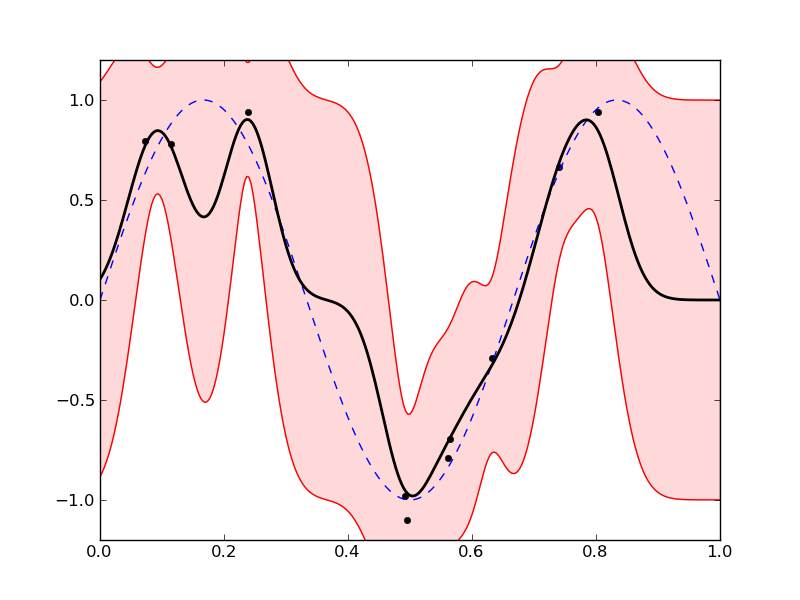
\includegraphics[width=3in]{gpr.png}\\$N=10$ points\end{center}
\end{frame}
\begin{frame}{Motivation for Gaussian Process Regression}
  \emph{Non-parametric} regression that quantifies uncertainty \\
  (pink regions represent 95\% CL)
  \begin{center}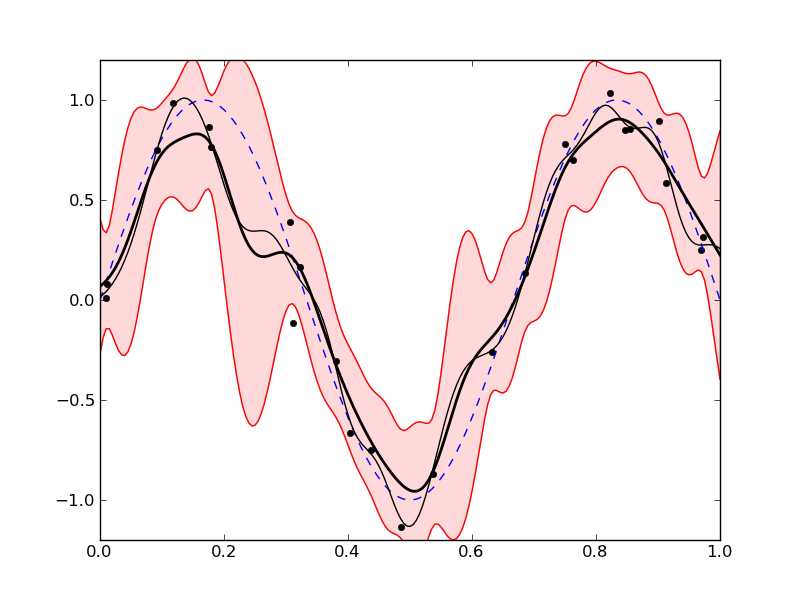
\includegraphics[width=3in]{gpr2.png}\\$N=25$ points\end{center}
\end{frame}
\begin{frame}{Computational Challenges in Gaussian Process Regression}
\begin{itemize}
\item The \emph{covariance matrix}
\begin{equation}
  K = \begin{bmatrix}
  k(x_1,x_1) & k(x_1, x_2) & \cdots & k(x_1,x_N) \\
  k(x_2,x_1) & k(x_2, x_2) & \cdots & k(x_2,x_N) \\
  \vdots & \vdots & \ddots & \vdots \\
  k(x_N,x_1) & k(x_N, x_2) & \cdots & k(x_N,x_N)
  \end{bmatrix}
\end{equation}
\item $k(x,x')$ is the \emph{covariance function}:
\begin{equation}
  k(x,x') = \sigma_f^2 \exp\left[\frac{-(x-x')^2}{2\ell^2}\right] + \sigma_n^2\delta(x,x'),
\end{equation}
\item Can predict mean and variance of $y_\ast$ at $x_\ast$:
\begin{equation}
\overline{y}_\ast = K_\ast K^{-1}\vec{y}
\end{equation}
\begin{equation}
\text{var}(y_\ast) = K_{\ast\ast}-K_\ast K^{-1}K_\ast^T
\end{equation}
%\item $\sigma_f$ is the maximum allowable covariance,
%\item $\ell$ is the length scale, 
%\item $\sigma_n$ is the Gaussian observation noise:
% \eq{y = f(x)+\mathcal{N}(0,\sigma_n^2)}
\end{itemize}
\end{frame}
\begin{frame}{Conjugate gradient method for matrix inversion}
Solving 
  \eq{\hat{K}\ket{x} = \ket{b} \implies \ket{x} = \hat{K}^{-1}\ket{b}}
is equivalent to minimization of
  \eq{f(\ket{x})=\frac{1}{2}\bra{x}\hat{K}\ket{x}-\bra{x}b\rangle}
CG method requires evaluation of $\hat{K}\ket{p}$ each iteration, if $\hat{K}$ is matrix of Gaussian kernels, $\hat{K}\ket{p}$ is equivalent to the \emph{Discrete Gauss Transform}
\begin{equation}
  G(y_j) = \sum_{i=1}^{N} p_i e^{-\abs{\abs{y_j-x_i}}^2/h^2}
\end{equation}
\end{frame}
\begin{frame}{The Improved Fast Gauss Transform}
\begin{itemize}
\item The \emph{Discrete Gauss Transform} 
\begin{equation}
  G(y_j) = \sum_{i=1}^{N} q_i e^{-\abs{\abs{y_j-x_i}}^2/h^2}
\end{equation}
\item $q_i$ are weight coefficients, 
\item $x_i$ are the centers of the Gaussians (``source'' points), 
\item $h$ is the bandwidth of the Gaussians.
\end{itemize}
Normally, with $N$ ``source'' points, and $M$ ``target'' points, we need to evaluate and sum $N\times M$ square exponentials. The Improved Fast Gauss Transform is an $\epsilon$-exact approximation that reduces complexity from $O(NM)$ to $O(M+N)$.  
\end{frame}

\begin{frame}{The Improved Fast Gauss Transform}
  Use $k$-center clustering (farthest point algorithm), greedy, $O(N)$
  \begin{center}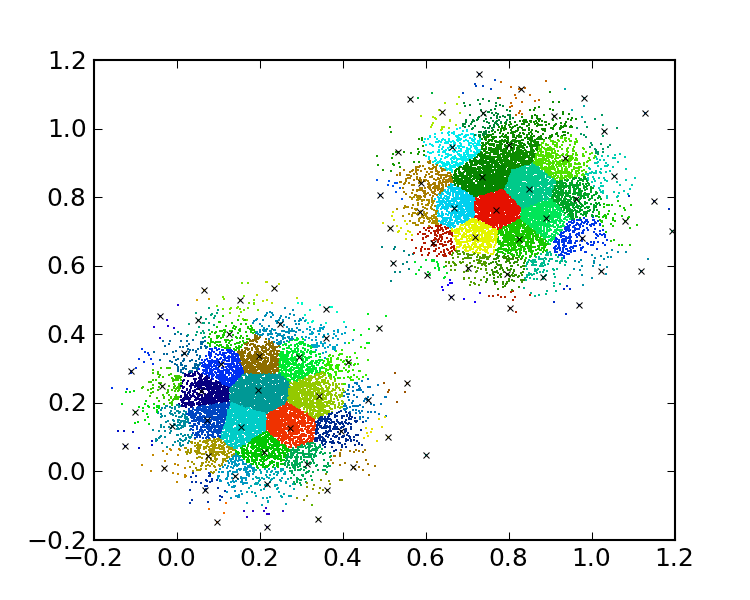
\includegraphics[width=3in]{clusters.png}\end{center}
  Efficient partitioning of space vs. multilevel grids from FMM, esp. in high dimensions
\end{frame}

\begin{frame}{The Improved Fast Gauss Transform}
  Sum of Gaussians approximated as (multinomial expansion as sum of monomials)
  \eq{G(y_j) &= \sum_{i=1}^{N} q_i e^{-\abs{\abs{y_j-x_i}}^2/h^2} \\
  &\approx \sum_{\abs{y_j-c_k}\leq h\rho_y} \sum_{\abs{\alpha}\leq p} C_\alpha^k e^{-\abs{y_j-c_k}^2/h^2}\left(\frac{y_j-c_k}{h}\right)^\alpha}
  Coefficients in \emph{graded lexicographical order}, Size of $\alpha$ is $\binom{p-1+d}{d}$
  \eq{C_\alpha^k=\frac{2^{\abs{\alpha}}}{\alpha!}\sum_{x_i\in S_k}q_ie^{-\abs{x_i-c_k}^2/h^2}\left(\frac{x_i-c_k}{h}\right)^\alpha}
\end{frame}

\begin{frame}{The Improved Fast Gauss Transform}
  \begin{center}
    Speedup: 83x vs. direct evaluation for 20k points\\
    \includegraphics[width=4in]{2D.pdf}\end{center}
\end{frame}
\begin{frame}{The Improved Fast Gauss Transform: Error Bound}
\begin{columns}[onlytextwidth]
  \begin{column}{0.4\textwidth}
  \begin{center}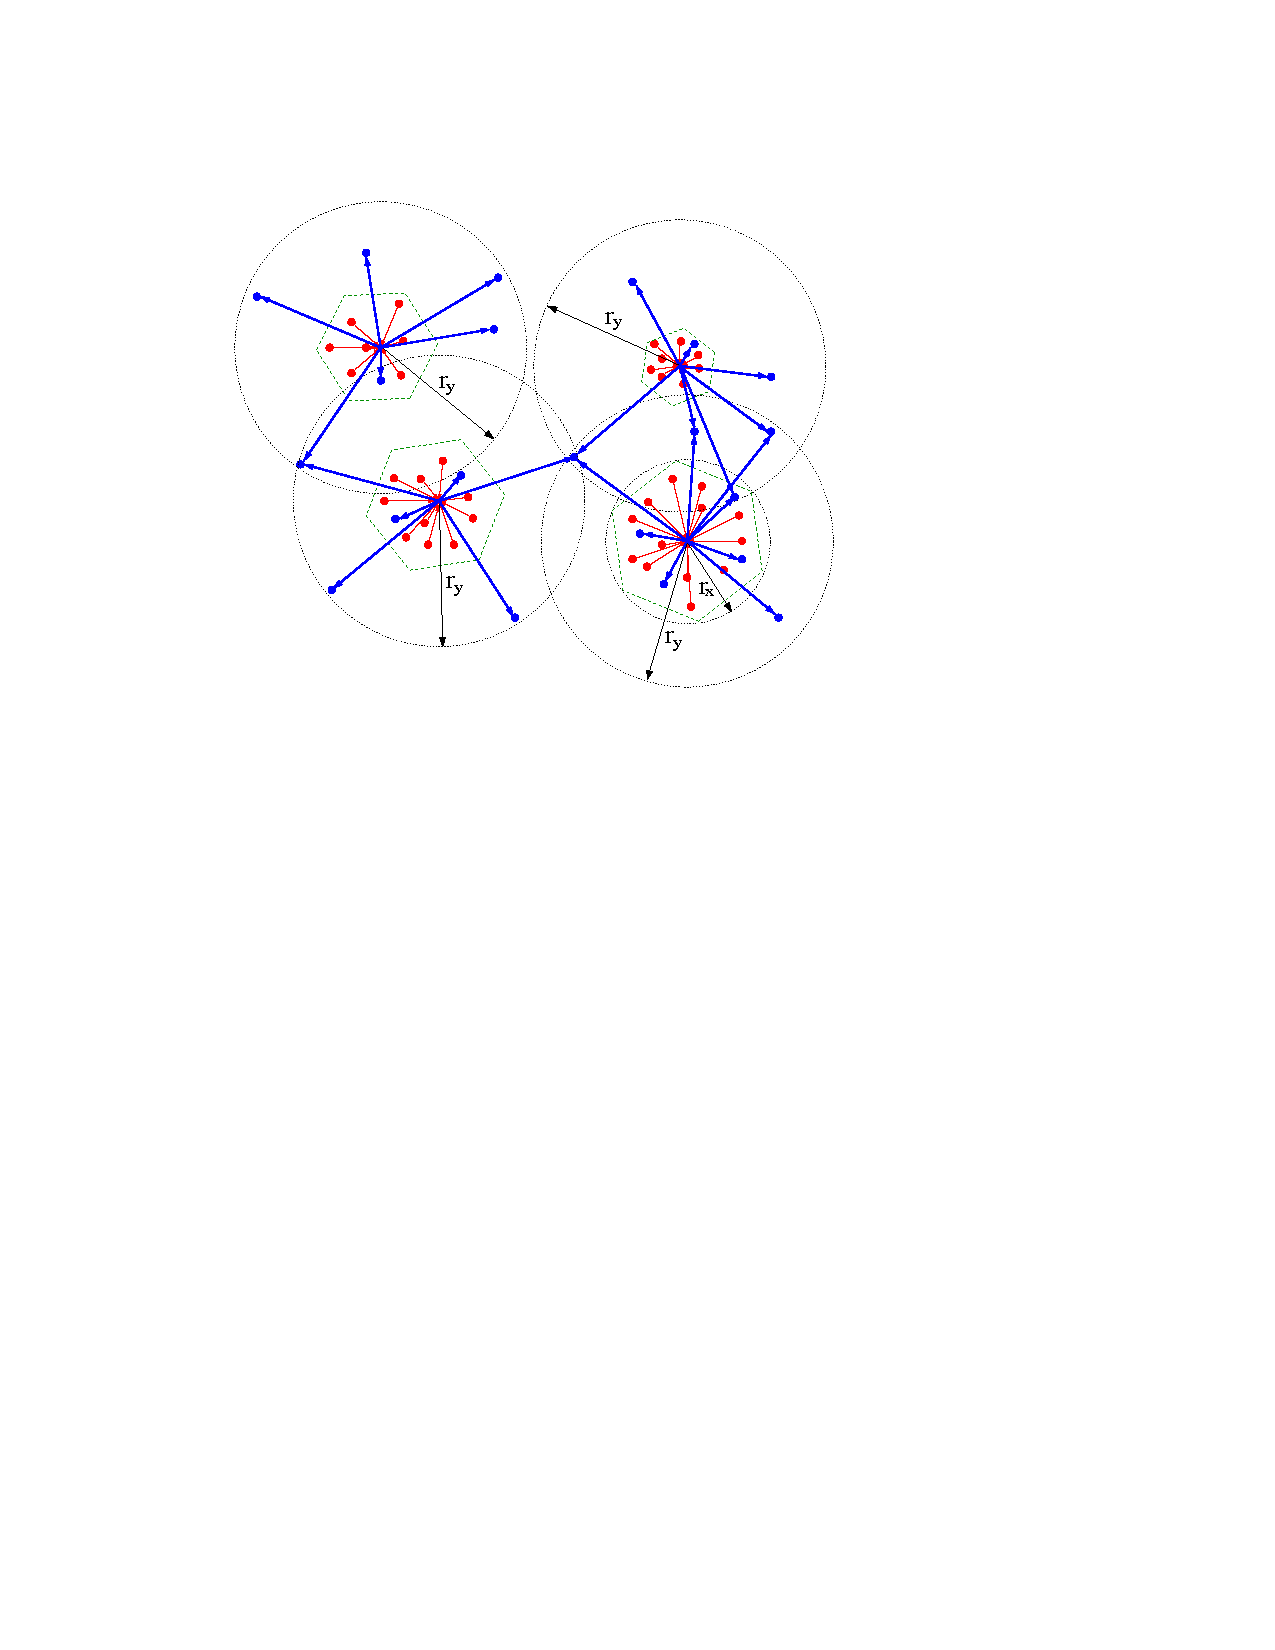
\includegraphics[width=2.5in]{trunc.pdf}\end{center}
  \end{column}
  \begin{column}{0.4\textwidth}
    Truncation term: \eq{\abs{E_T}\leq \frac{2^p}{p!}\left(\frac{r_xr_y}{h}\right)^p}
	Cutoff term: \eq{\abs{E_C}\leq e^{-r_y^2/h^2}}
  \end{column}
\end{columns}
    \eq{\text{Total: }\abs{E(y)}\leq Q\left(\frac{2^p}{p!}\left(\frac{r_xr_y}{h}\right)^p + e^{-r_y^2/h^2}\right)}
\end{frame}
\begin{frame}{Applying IFGT to GPR} 
  \begin{itemize}
    \item Rewrite $K^{-1}\vec{y}$ as CG minimization problem
      \begin{itemize}
        \item Numerical experiments show that CG minimization without IFGT use 15-30 weak scaling with $N$
        \begin{center}
          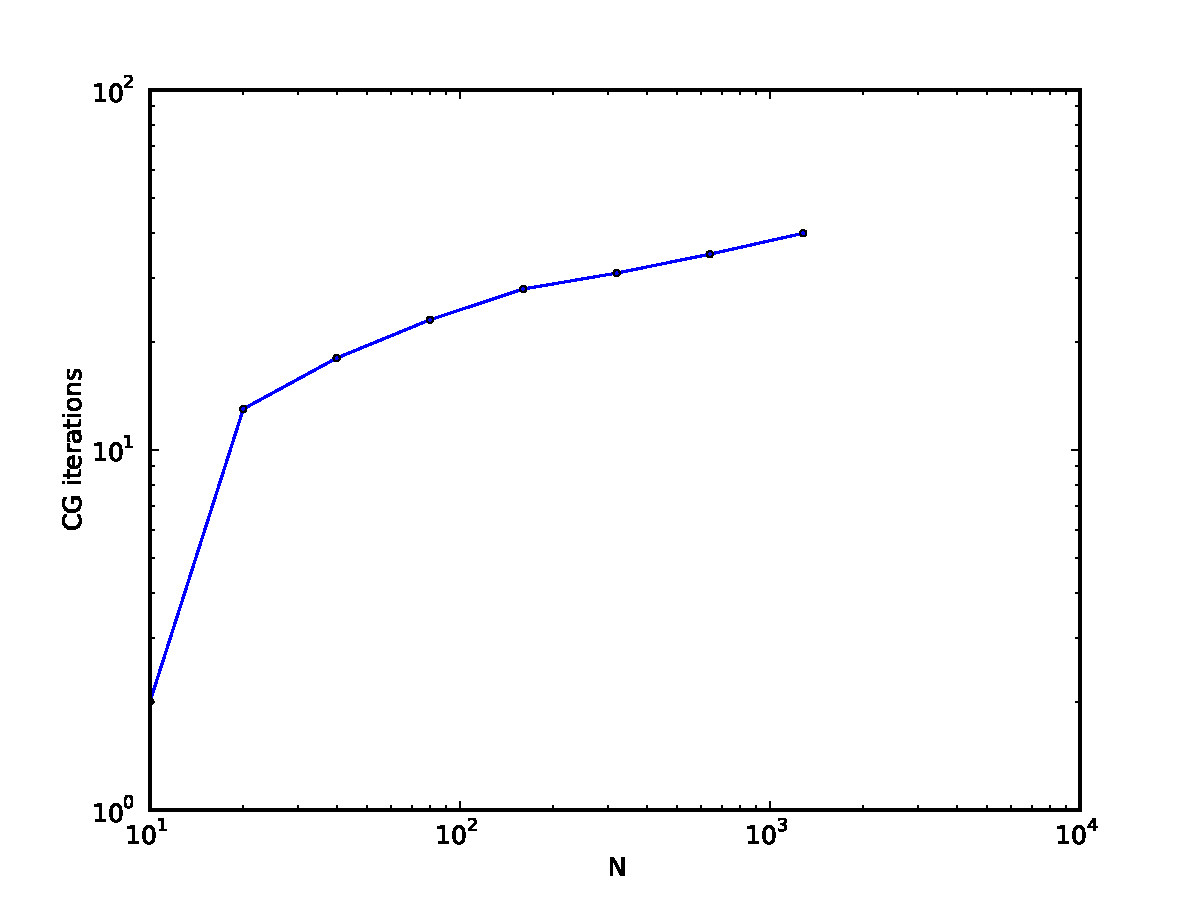
\includegraphics[width=1.5in]{cgtrend.pdf}
          \end{center}
      \end{itemize}
    \item Re-frame matrix-vector multiplication $K\ket{p}$ as a discrete Gauss transform
    \begin{itemize}
      \item i.e., $N\times N$ matrix $\to$ $N$ source points, evaluated at $N$ target points with weights given by $p_i$, $i=1,\dots,N$. 
    \end{itemize}
    \end{itemize}
\end{frame}
\begin{frame}{Applying IFGT to GPR}
\eq{K\ket{p} &= 
  \begin{bmatrix}
  k(x_1,x_1) & k(x_1, x_2) & \cdots & k(x_1,x_N) \\
  k(x_2,x_1) & k(x_2, x_2) & \cdots & k(x_2,x_N) \\
  \vdots & \vdots & \ddots & \vdots \\
  k(x_N,x_1) & k(x_N, x_2) & \cdots & k(x_N,x_N)
  \end{bmatrix}
\begin{bmatrix}p_1\\p_2\\\vdots\\p_N\end{bmatrix} \\
&= 
\begin{bmatrix}
\sum_{i=1}^N p_i k(x_1, x_i)\\
\sum_{i=1}^N p_i k(x_2, x_i)\\
\vdots \\
\sum_{i=1}^N p_i k(x_N, x_i)
\end{bmatrix} = \begin{bmatrix}
G(x_1) \\
G(x_2) \\
\vdots \\
G(x_N)
\end{bmatrix}}
\eq{\text{where } G(x_j) = \sum_{i=1}^N \underbrace{(p_i \sigma_f^2)}_{q_i} \exp\left[\frac{-(x_j-x_i)^2}{h^2}\right], \quad h = \sqrt{2}\ell}
Can evaluate $K\ket{p}$ in $O(N+N)$ instead of $O(N^2)$ on $G(\vec{x})$.
\end{frame} 

\begin{frame}{Implementation}
\begin{itemize}
\item To evaluate IFGT: \\
\small{
\texttt{IFGT ifgt(sources, weights, 0.1, 15,  0.3, 2);} \\
\texttt{ifgt.evaluate(sources, result);}}
\parbox{3in}{}
\item To evaluate $K\ket{x}$:\\
\texttt{Vector Kx;} \\
\texttt{Vector x(N, sigma\_f * sigma\_f);} \\
\texttt{IFGT KxIFGT(sources, x, sqrt(2) * length, degree, radius, cutoff);} \\
\texttt{KxIFGT.evaluate(sources, Kx);}
\end{itemize}
\begin{itemize}
  \item C++, no special libraries. 
  \item View project on github \\
  \small{\url{https://github.com/chi-feng/ifgt-gpr/tree/master/src}}
  \end{itemize}  
\end{frame}

\begin{frame}{Future Work}
\begin{itemize}
  \item Apply IFGT to \emph{hyperparameter selection} (choose $\sigma_f, \sigma_n, \ell$ to maximize posterior likelihood), i.e. maximize:
  \eq{\log p(\vec{y}|\vec{x},\sigma_f, \sigma_n,\dots) = -\frac{1}{2}\vec{y}^T K^{-1}\vec{y}-\frac{1}{2}log\abs{K}}
  \item Apply IFGT to other covariance kernels.
  \begin{itemize}
    \item Multiple length-scales (to capture oscillations)
    \eq{ k(x,x') = \sigma_f^2 \exp\left[\frac{-(x-x')^2}{2\ell_1^2}\right] + \sigma_f^2 \exp\left[\frac{-(x-x')^2}{2\ell_2^2}\right]}
    \end{itemize}
  \item Apply IFGT-accelerated Gaussian Process Regression to interesting problems, e.g. level sets and classification of high-dimensional data. 
\end{itemize}
\end{frame}

\begin{frame}{Bibliography}
  \begin{itemize}
  \item Changjiang Yang and Duraiswami, R. and Gumerov, N.A. and Davis, L., \emph{Computer Vision, 2003. Proceedings. Ninth IEEE International Conference}, 
  ``Improved fast gauss transform and efficient kernel density estimation,'' (2003)
  \item M. Ebden, \emph{Gaussian Processes for Regression: A Quick Introduction} (2008) \url{http://www.robots.ox.ac.uk/~mebden/reports/GPtutorial.pdf}
  \item Rasmussen, C. and C. Williams (2006). \emph{Gaussian Processes for Machine Learning.} MIT Press.
  \end{itemize}
  \end{frame}
\end{document}